\documentclass[../xlapes02]{subfiles}
\begin{document}
    \chapter{Implementation}\label{ch:implementation}


    \section{Data Engineering}\label{sec:data-engineering}
    Data engineering is critical in AI to ensure quality, preparation, integration, scalability, governance, and performance optimization of models. It involves cleaning, organizing, and transforming data for accurate model training, handling large volumes of data, and adhering to regulations. High-quality data and effective data engineering processes are crucial for developing reliable and scalable AI models. In this section, we describe our approach to data engineering used for Portfolio Management by first defining the data collection~\cref{subsec:data-collection}, dataset preprocessing~\cref{subsec:dataset-preprocessing}, and dataset splitting~\cref{subsec:dataset-splitting}.

    \subsection{Data Collection}\label{subsec:data-collection}
    Raw data was gathered from these sources:
    \begin{itemize}
        \item Yahoo Finance: \url{https://finance.yahoo.com/}
        \item Financial Modeling Prep: \url{https://financialmodelingprep.com/}
    \end{itemize}
    these sources provide financial data for 60000+ tickers, with a history of over 30 years.

    We focus on tickers (companies) from Dow Jones Industrial Average (DJIA), which includes 30 companies. More about which companies are included in DJIA, you can see~\cite{enwiki:1141766585}.

    \subsection{Data Preprocessing}\label{subsec:dataset-preprocessing}
    In this section, we describe our approach to dataset preprocessing by first defining the data cleaning~\cref{subsubsec:data-cleaning}, feature engineering~\cref{subsubsec:feature-engineering}.

    \subsubsection{Data Cleaning}\label{subsubsec:data-cleaning}
    We use the following company data in our datasets: prices, financial statements and technical indicators. Prices are used to calculate earnings, financial statements are used to calculate fundamentals. Fundamental indicators and technical analysis indicators are used for feature engineering. Data cleaning is done by removing rows with missing values. Missing values are replaced by the average of the column. If data is completely missing on a date, all rows up to that next date are removed for the other companies. This can happen mostly for companies that are not listed in any time period. Data cleaning is performed for all data sets.

    \subsection{Feature Engineering}\label{subsubsec:feature-engineering}
    In this subsection, we describe our approach to feature engineering which we divide into three parts: fundamental analysis, described in~\cref{subsubsec:fundamental-analysis}, technical analysis, described in~\cref{subsubsec:technical-analysis}, and combined fundamental and technical analysis is described in~\cref{subsubsec:combined-fundamental-and-technical-analysis}.

    \subsubsection{Fundamental Analysis}\label{subsubsec:fundamental-analysis}
    Fundamental data means the basic and essential information about a company or asset that is used to analyse its financial health, performance and valuation. It includes data relating to the company's financial statements, business operations, management team, industry and economic environment. Fundamental data is commonly used by investors, analysts and financial professionals to make investment decisions and to assess the intrinsic value of an asset. For fundamental analysis, we use the following income statement, balance sheet and cash flow for each company. For our first dataset, we use the following financial ratios: operating margin, net profit margin. Return on assets (ROA), Return on equity (ROE), Current ratio, Cash ratio, Inventory turnover, Accounts receivable turnover, Accounts payable turnover, Debt ratio, Debt to equity ratio, Price to earnings ratio (PE Ratio), Price to book value ratio (PB Ratio) and Dividend yield. We will now describe each of these ratios.

%    \paragraph{Net Income}\label{par:net-income}
%    Net income is the amount of money a company makes after subtracting all expenses and taxes. It is also known as the bottom line because it is found on the last line of a company's income statement. The Net Income is calculated as:
%    \begin{equation}
%        \begin{split}
%            Net\ Income&=R-COGS-E-I-T\\
%        \end{split}
%    \end{equation}
%    where $R$ is the revenue, $COGS$ is the cost of goods sold, $E$ is the expenses, $I$ is the interest, and $T$ is the taxes.

    \paragraph{Operating Margin}\label{par:operating-margin}
    The Operating Margin represents how efficiently a company is able to generate profit through its core operations. It is expressed on a per-sale basis after accounting for variable costs but before paying any interest or taxes (EBIT). Higher margins are considered better than lower margins and can be compared between similar competitors but not across different industries. To calculate the operating margin, divide operating income (earnings) by sales (revenues)~\cite{investopedia-operating-margin}:
    \begin{equation}
        Operating\ Margin=\frac{Operating\ Income}{Net\ Sales}
    \end{equation}
    where $Operating\ Income$ refers to the adjusted revenue of a company after all expenses of operation and depreciation are subtracted. Expenses of operation or operating expenses are simply the costs incurred in order to keep the business running~\cite{investopedia-operating-income}. $Net\ Sales$ may be defined as money paid by customers. Sales are a company's core revenue for a given period~\cite{investopedia-net-sales}. Operating margin, expressed as a percentage, indicates the earnings generated from each dollar of sales after accounting for direct costs. Higher margins mean more profit from each sale~\cite{investopedia-operating-margin}.

    \paragraph{Net Profit Margin}\label{par:net-profit-margin}
    The Net Profit Margin is a profitability ratio that measures a company's ability to generate income after all expenses and taxes have been paid $Net\ Income$. It is calculated by dividing a company's $Net\ Income$, by its $Total\ Revenue$~\cite{investopedia-net-income, investopedia-revenue}. The net profit margin is a measure of how much of each dollar of revenue is left over after all expenses and taxes have been paid. It is a useful metric for comparing the profitability of different companies in the same industry. The higher the net profit margin, the more profitable a company is. The net profit margin is calculated as follows~\cite{investopedia-net-profit-margin}:
    \begin{equation}
        \begin{split}
            Net\ Profit\ Margin&=\frac{Net\ Income}{Total\ Revenue}\\
        \end{split}
    \end{equation}

    \paragraph{Return On Assets}\label{par:return-on-assets}
    Return on assets (ROA) is a measure of profitability that calculates how much profit a company makes with the money it has invested. It is calculated by dividing a company's $Net\ Income$ by its $Total\ Assets$~\cite{investopedia-net-income, investopedia-assets}. The higher the ROA, the more profitable a company is. The ROA is calculated as follows~\cite{investopedia-return-on-assets}:
    \begin{equation}
        \begin{split}
            Return\ On\ Assets&=\frac{Net\ Income}{Total\ Assets}\\
        \end{split}
    \end{equation}

    \paragraph{Return On Equity}\label{par:return-on-equity}
    Return on equity (ROE) is a measure of profitability that calculates how much profit a company makes with the money shareholders have invested. It is calculated by dividing a company's $Net\ Income$ by its $Average\ Shareholders'\ Equity$~\cite{investopedia-net-income}. The higher the ROE, the more profitable a company is. The ROE is calculated as follows~\cite{investopedia-return-on-equity}:
    \begin{equation}
        \begin{split}
            Return\ On\ Equity&=\frac{Net\ Income}{Average\ Shareholders'\ Equity}\\
        \end{split}
    \end{equation}

    \paragraph{Current Ratio}\label{par:current-ratio}
    The current ratio is a liquidity ratio that measures a company's ability to pay short-term and long-term obligations. It is calculated by dividing a company's $Current\ Assets$ by its $Current\ Liabilities$~\cite{investopedia-current-assets, investopedia-current-liabilities}. The higher the current ratio, the more capable a company is of paying its short-term and long-term obligations. The current ratio is calculated as follows~\cite{investopedia-current-ratio}:
    \begin{equation}
        \begin{split}
            Current\ Ratio&=\frac{Current\ Assets}{Current\ Liabilities}\\
        \end{split}
    \end{equation}
    where $Current\ Assets$ is $Cash\&Equivalent+Short\ Term\ Investments+Account\ Receivable+Inventory$. If the $Current Ratio < 1$ that is a sign of financial distress, and the company could be unable to pay its short-term and long-term obligations. On the other hand, if the $Current Ratio$ is too high, it could be a sign that the company is not using its assets efficiently.

    \paragraph{Quick Ratio}\label{par:quick-ratio}
    The quick ratio is a liquidity ratio that measures a company's ability to pay short-term obligations. It is calculated by dividing a company's $Quick\ Assets$ by its $Current\ Liabilities$. The higher the quick ratio, the more capable a company is of paying its short-term obligations. The quick ratio is calculated as follows~\cite{investopedia-quick-ratio}:
    \begin{equation}
        \begin{split}
            Quick\ Ratio&=\frac{Quick\ Assets}{Current\ Liabilities}\\
        \end{split}
    \end{equation}
    where $Quick\ Ratio$ is $Cash\&Equivalents+Marketable\ Securities+Net\ Accounts\ Receivable$. If the company would have a $Quick Ratio < 1$, it would be a sign of financial distress, and the company would be unable to pay its short-term obligations.

    \paragraph{Cash Ratio}\label{par:cash-ratio}
    The cash ratio is a liquidity ratio that measures a company's ability to pay short-term obligations. It is calculated by dividing a company's $Cash\&Equivalents$ by its $Current\ Liabilities$. The higher the cash ratio, the more capable a company is of paying its short-term obligations. The cash ratio is calculated as follows~\cite{investopedia-cash-ratio}:
    \begin{equation}
        \begin{split}
            Cash\ Ratio&=\frac{Cash\&Equivalent}{Current\ Liabilities}\\
        \end{split}
    \end{equation}

    \paragraph{Inventory Turnover}\label{par:inventory-turnover}
    The inventory turnover ratio is a measure of how efficiently a company is managing its inventory. It is calculated by dividing a company's $COGS$ by its $Average\ Value\ of\ Inventory$. The higher the inventory turnover ratio, the more efficiently a company is managing its inventory. The inventory turnover ratio is calculated as follows~\cite{investopedia-inventory-turnover}:
    \begin{equation}
        \begin{split}
            Inventory\ Turnover&=\frac{COGS}{Average\ Value\ of\ Inventory}\\
        \end{split}
    \end{equation}
    where $COGS$ is an acronym for Cost of Goods Sold, which is also known as the cost of sales. To calculate inventory turnover, analysts use COGS instead of sales because inventory is valued at cost. Some companies may use sales instead of COGS, which can inflate the ratio.

    \paragraph{Receivables Turnover}\label{par:receivables-turnover}
    The receivables turnover ratio is a measure of how efficiently a company is managing its accounts receivable. It is calculated by dividing a company's $Net\ Credit\ Sales$ by its $Average\ Accounts\ Receivable$. The higher the receivables turnover ratio, the more efficiently a company is managing its accounts receivable. The receivables turnover ratio is calculated as follows~\cite{investopedia-recievables-turnover}:
    \begin{equation}
        \begin{split}
            Receivables\ Turnover&=\frac{Net\ Credit\ Sales}{Average\ Accounts\ Receivable}\\
        \end{split}
    \end{equation}
    where $Net\ Credit\ Sales$ is the total sales minus the cash sales. The receivables turnover ratio measures a company's ability to collect accounts receivable. A low ratio suggests difficulty collecting payments, while a high ratio may indicate efficient collection, but may also suggest lost sales due to not extending credit long enough.

    \paragraph{Payables Turnover}\label{par:payables-turnover}
    The accounts payable turnover ratio is a short-term liquidity measure used to quantify the rate at which a company pays off its suppliers. Accounts payable turnover shows how many times a company pays off its accounts payable during a period. It is calculated by dividing a company's total suply purchases by its average accounts payable. The higher the payables turnover ratio, the more efficiently a company is managing its accounts payable. The payables turnover ratio is calculated as follows~\cite{investopedia-payables-turnover}:
    \begin{equation}
        \begin{split}
            Payables\ Turnover&=\frac{TSP}{(BAP+EAP)/2}\\
        \end{split}
    \end{equation}
    where $TSP$ is the total supply purchase, $BAP$ is the beginning accounts payable, and $EAP$ is the ending accounts payable. If the payables turnover ratio is too low, it could be a sign that company has trouble paying its suppliers. If the payables turnover ratio is too high, it could be a sign that the company is not using its assets efficiently.

    \paragraph{Debt Ratio}\label{par:debt-ratio}
    The debt ratio is a measure of a company's financial leverage. It is calculated by dividing a company's $Total\ Liabilities$ by its $Total\ Assets$. The higher the debt ratio, the more debt a company is using to finance its assets. The debt ratio is calculated as follows~\cite{investopedia-debt-ratio}:
    \begin{equation}
        \begin{split}
            Debt\ Ratio&=\frac{Traditional\ Debt+(Accounts\ Payable+Taxes\ Payable)}{Total Assets}\\
        \end{split}
    \end{equation}
    A lower debt ratio is preferable. A Debt Ratio greater than 1.0 implies that a company has more debt than assets, whereas a Debt Ratio less than 1 indicates that a company has more assets than debt.

    \paragraph{Debt Equity Ratio}\label{par:debt-equity-ratio}
    The Debt to Equity Ratio (D/E) is a measure of a company's financial leverage. It is calculated by dividing a company's $Total\ Liabilities$ by its $Total\ Equity$. The higher the debt equity ratio, the more debt a company is using to finance its assets. The debt equity ratio is calculated as follows~\cite{investopedia-debt-equity-ratio}:
    \begin{equation}
        \begin{split}
            Debt\ Equity\ Ratio&=\frac{Total\ Liabilities}{Total\ Equity}\\
        \end{split}
    \end{equation}
    where $Total\ Liabilities$ are $Traditional\ Debt+(Accounts\ Payable+Taxes\ Payable)$. A lower $Debt\ Equity\ Ratio$ is preferable.

    \paragraph{Price Earnings Ratio}\label{par:price-earnings-ratio}
    The Price Earnings Ratio (P/E) is a measure of a company's value relative to its earnings. It is calculated by dividing a company's $Stock\ Price$ by its $Earnings\ per\ Share$. The higher the price earnings ratio, the more expensive a company's stock is relative to its earnings. The price earnings ratio is calculated as follows~\cite{investopedia-price-earnings-ratio}:
    \begin{equation}
        \begin{split}
            Price\ Earnings\ Ratio&=\frac{Stock\ Price}{Earnings\ Per\ Share}\\
        \end{split}
    \end{equation}
    High P/E implies investors anticipate greater future earnings growth compared to low P/E companies. A low P/E can signal undervaluation or exceptional performance relative to past trends.

    \paragraph{Price Book Value Ratio}\label{par:price-book-value-ratio}
    The Price Book Value Ratio (P/B) is a measure of a company's value relative to its book value. It is calculated by dividing a company's $Stock\ Price$ by its $Book\ Value\ per\ Share$. The higher the price book value ratio, the more expensive a company's stock is relative to its book value. The price book value ratio is calculated as follows~\cite{investopedia-price-book-value-ratio}:
    \begin{equation}
        \begin{split}
            Price\ Book\ Value\ Ratio&=\frac{Stock\ Price\ per\ Share}{Book\ Value\ per\ Share}\\
        \end{split}
    \end{equation}
    A low P/B ratio, especially below one, could signal undervaluation where stock price is lower than the value of the company's assets. A P/B ratio above one indicates the stock is trading at a premium to book value, potentially overvalued. For instance, a P/B ratio of three means the stock trades at three times book value.

    \paragraph{Dividend Yield}\label{par:dividend-yield}
    The dividend yield, expressed as a percentage, is a financial ratio (dividend/price) that shows how much a company pays out in dividends each year relative to its stock price. It is calculated by dividing a company's $Annual\ Dividend$ by its $Stock\ Price$. It is a measure of a company's profitability. The higher the dividend yield, the more profitable a company is. The dividend yield is calculated as follows~\cite{investopedia-dividend-yield}:
    \begin{equation}
        \begin{split}
            Dividend\ Yield&=\frac{Annual\ Dividend}{Stock\ Price}\\
        \end{split}
    \end{equation}

    \subsubsection{Technical Analysis}\label{subsubsec:technical-analysis}
    Technical analysis is a method used in financial markets such as stocks, currencies and commodities to analyse historical price data and identify patterns, trends and signals that can be used to make trading decisions. Technical analysis is based on the belief that historical price and volume data can provide insight into future price movements and focuses primarily on the analysis of price charts and other technical indicators. In this section we present the technical indicators that we have selected based on the correlation between all indicators.


    \section{Feature Selection}\label{sec:feature-selection}
    Technical indicators are calculated based on historical share price data. To calculate these indicators, the Finta framework was used, which provides more than 100 different functions for calculating technical indicators. The framework is written in Python and is available on GitHub~\cite{finta}.

    First, we calculate all technical indicators for all stocks in the dataset. Then we calculate the correlation matrix between all indicators. The correlation matrix is a square matrix that contains the correlation coefficient between all pairs of indicators. The correlation coefficient is a measure of the linear correlation between two variables. The decay coefficient of the correlation is $0.5$, that is, if $|\rho| > 0.5$, then we omit one or the other variable, where $\rho$ is the correlation between the two variables, defined in~\cref{eq:corr}. Since the image for all indicators is too large, we only show the correlation matrix for the uncorrelated indicators (we filtered out the correlated indicators) that we used in the dataset, see ~\cref{fig:ta_correlation_matrix_uncorrelated_indicators}.
    \begin{figure}[h]
        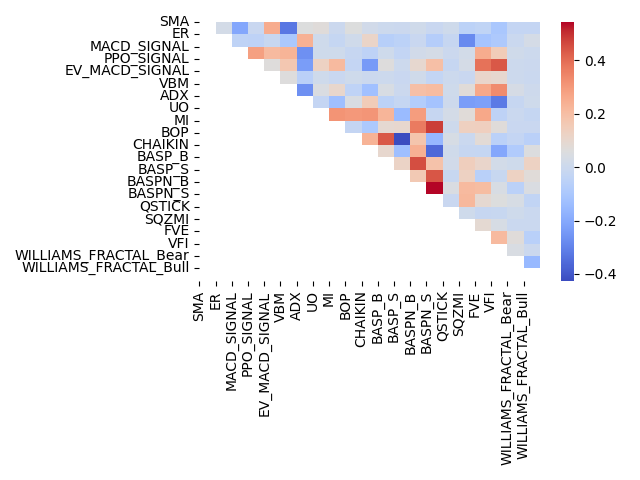
\includegraphics[width=0.95\linewidth]{image/ta_correlation_matrix_uncorrelated_indicators}
        \centering
        \caption{Correlation matrix of technical indicators after removing correlated indicators.}
        \label{fig:ta_correlation_matrix_uncorrelated_indicators}
    \end{figure}
    the only part above the diagonal is shown, since the correlation matrix is symmetric. The correlation matrix shows that the indicators are not correlated with each other. The correlation matrix is calculated using \emph{Pearson Method} as follows~\cite{enwiki:1146097966}:
    \begin{equation}
        \label{eq:corr}
        \begin{split}
            \rho&=\frac{\sum_{i=1}^{n}(x_i-\bar{x})(y_i-\bar{y})}{\sqrt{\sum_{i=1}^{n}(x_i-\bar{x})^2}\sqrt{\sum_{i=1}^{n}(y_i-\bar{y})^2}}\\
        \end{split}
    \end{equation}

    \subsubsection{Combined Fundamental and Technical Analysis}\label{subsubsec:combined-fundamental-and-technical-analysis}
    Combining datasets is a process in which two or more datasets are merged or joined together to create a new dataset that contains information from both. In this case, the combined fundamental and technical analysis involves combining features from both fundamental analysis~\cref{subsubsec:fundamental-analysis} and technical analysis, described in~\cref{subsubsec:technical-analysis}.

    By combining fundamental and technical analysis, we can create a more comprehensive and accurate picture of the market. For example, fundamental analysis can help identify undervalued or overvalued assets, while technical analysis can help identify trends and potential buying or selling opportunities. The specific features used in the combined analysis can depend on the specific dataset and the machine learning task being performed. However, we leave all features from both analysis.

    \subsection{Dataset Splitting}\label{subsec:dataset-splitting}
    Dataset splitting refers to the process of dividing a dataset into two or more subsets to be used for training and testing machine learning models. In this particular case, the dataset is a time series data, which means that the order of the data points is important, and the dataset must be split in a way that preserves the temporal ordering.

    The division coefficient of $0.6$ means that $60\%$ of the dataset will be used for training, and $40\%$ will be used for testing. This is a common split ratio, but the exact ratio can vary depending on the size and complexity of the dataset, as well as the specific machine learning task being performed.

    In this case, since the dataset consists of daily data and spans a period from 2008-03-20 to 2022-12-16, we can split it based on time. The first $60\%$ of the data, starting from the beginning of the dataset on 2008-03-20, will be used for training, and the remaining $40\%$ of the data will be used for testing. This ensures that the model is trained on past data and tested on future data, which is a more realistic scenario.

    The training set will be used to train the machine learning model, while the testing set will be used to evaluate its performance. By splitting the dataset, we can avoid overfitting, which is when the model memorizes the training data and performs poorly on new, unseen data. The testing set provides a way to measure the model's generalization performance on unseen data, which is an important metric for evaluating the model's effectiveness.

    Dataset splitting is an important step in machine learning that helps ensure that the model is trained and tested on different subsets of data. In this case, the dataset is split into training and testing sets based on time, with $60\%$ of the data used for training and $40\%$ used for testing. This split ensures that the model is evaluated on unseen data and can generalize well to new data.

\end{document}
